\documentclass{labo}

\usepackage{charter}
\usepackage[utf8x]{inputenc}
\usepackage[T1]{fontenc}
\usepackage{ucs}
\usepackage{amsthm} %numéroter les questions
\usepackage[frenchb]{babel}
\usepackage{datetime}
\usepackage{xspace} % typographie IN
\usepackage{hyperref}% hyperliens
\usepackage[all]{hypcap} %lien pointe en haut des figures
\usepackage[french]{varioref} %voir x p y
\usepackage{fancyhdr}% en têtes
\usepackage[]{graphicx} %include pictures
% \usepackage{pgfplots}
\usepackage[americanresistors,siunitx]{circuitikz}
\usepackage[]{gnuplottex}
\usepackage{ifthen}
\usepackage{mathastext} % math as standfard text : units are respecting typography conventions.
\usepackage[]{subfig}
\usepackage[]{attachfile}
\usepackage{tikz}
\usetikzlibrary{babel,positioning,calc}
\usepackage{siunitx}
\usepackage{amssymb}
\usepackage{xcolor}
\usepackage{float}
\usepackage[normalem]{ulem}
\usepackage{todonotes}

%%%%%%%%%%%%
% Tables
%%%%%%%%%%%%
\usepackage{booktabs}
\renewcommand{\arraystretch}{1.1} % Opens up the table a tad
\usepackage{multicol}
\usepackage{multirow}

\newboolean{koriG}
\ifx\koriG\undefined
\correction{false}
\else
\correction{true}
\fi

\newcommand{\itgv}[1]{\ifthenelse{\boolean{corrige}}{{\color{blue}#1}}{}} %si corrigé vrai...
\newcommand{\ifgv}[1]{\ifthenelse{\boolean{corrige}}{}{#1}} %si corrigé vrai...

% \correction{false}
%\correction{true}

\definecolor{darkblue}{rgb}{0,0,0.5}

%% fancy header & foot
\pagestyle{fancy}
\lhead{[EOSI40] Instrumentation labs\\ Lab 1: First look at LabView}
\rhead{v0.9.0 \\ page \thepage}
\chead{\ifthenelse{\boolean{corrige}}{Corrigé}{}}
\cfoot{}
%%

\author{GEI}


\setlength{\parindent}{0pt}


%from SO: kinky cross for wires
\tikzset{
  declare function={% in case of CVS which switches the arguments of atan2
    atan3(\a,\b)=ifthenelse(atan2(0,1)==90, atan2(\a,\b), atan2(\b,\a));},
  kinky cross radius/.initial=+.125cm,
  @kinky cross/.initial=+, kinky crosses/.is choice,
  kinky crosses/left/.style={@kinky cross=-},kinky crosses/right/.style={@kinky cross=+},
  kinky cross/.style args={(#1)--(#2)}{
    to path={
      let \p{@kc@}=($(\tikztotarget)-(\tikztostart)$),
          \n{@kc@}={atan3(\p{@kc@})+180} in
      -- ($(intersection of \tikztostart--{\tikztotarget} and #1--#2)!%
             \pgfkeysvalueof{/tikz/kinky cross radius}!(\tikztostart)$)
      arc [ radius     =\pgfkeysvalueof{/tikz/kinky cross radius},
            start angle=\n{@kc@},
            delta angle=\pgfkeysvalueof{/tikz/@kinky cross}180 ]
      -- (\tikztotarget)}}}


\begin{document}
\tptitle{}{Lab 1: First look at LabView}

Through the following labs, you will get acquainted with LabView from National Instruments.
There are \href{https://www.ni.com/docs/en-US/bundle/labview/page/lvconcepts/labview_fundamentals.html}{detailed documentation online} on NI's website.

\section{MyFirstVI}
LabView programs are called ``Virtual Instruments'' (VI) and comprise three elements:
\begin{enumerate}
	\item The front view
	\item The diagram
	\item The icon/connector
\end{enumerate}

In a program, the inputs are defined as ``commands'' and the outputs to display as ``indicators''.

Build a program that sum two numbers and displays the result.

To modify the icon and the connector, click on the following elements from Figure~\ref{fig:mod-icon-conn}.

\begin{figure}[h!]
\centering
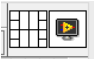
\includegraphics[]{mod-icon-conn.png}
\caption{}\label{fig:mod-icon-conn}
\end{figure}


\section{Celsius to Fahrenheit conversion}
Build a program that can convert a temperature from $x$ Celsius degrees to $y$ Fahrenheit degrees following this relation: $$y = x \cdot \frac{9}{5} + 32$$

Save your VI and make an appropriate icon and connector.



\section{Display panel}
Use your VI from the previous question to create a voltage/temperature converter with a scale selection.
Use the random number generator module to simulate a measure and multiply that number by 100 to obtain a value in Celsius degrees.
Add a switch button to choose the display scale.
The front view might look like Figure~\ref{fig:display-panel}.

\begin{figure}[h!]
\centering
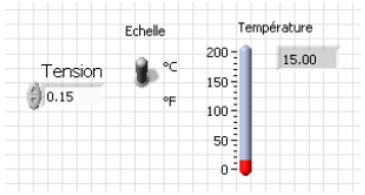
\includegraphics[width=.6\textwidth]{display-panel.png}
\caption{}\label{fig:display-panel}
\end{figure}




\section{Random number generator}
Build a program that generates a random number and then displays it on a rolling graph.
The delay before a new value appears must be parametric.
You need a \texttt{while} loop and the \texttt{delay} function to specify the time interval between two number generations, i.e. the time the program needs to wait between the execution of successive loops.
An on/off button must allow to start/stop the experiment.

The front view to obtain should look like Figure~\ref{fig:rng}.

\begin{figure}[h!]
\centering
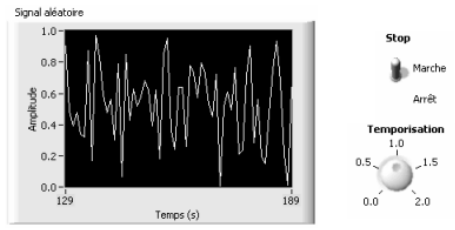
\includegraphics[width=.7\textwidth]{rng.png}
\caption{}\label{fig:rng}
\end{figure}



\section{Sinusoidal signal generator and threshold detection}
Simulate a sinusoidal signal with a random amplitude and frequency.
Display the signal on a rolling graph.
Implement a threshold detection: if the signal is above 7 volts, trigger an alert by lighting up an LED in the front view.
Display this alert on the graph as well.

The frequency ranges from 1 to 20Hz and the amplitude ranges from 0 to 10V.

Similar to exercise 4, design a variable delay between two successive signal generations.



\section{Bonus}
Explore how to keep logs of the experiment by saving the results in a file.
What are the LabView objects that allow such features?



% \Question{}{}
\end{document}
